\begin{question}
\noindent A research satellite tracks a rare specimen on a grid map of a nature reserve.
At 06:00, the specimen is marked at point $P(-4, 1)$ on the grid.

\begin{center}
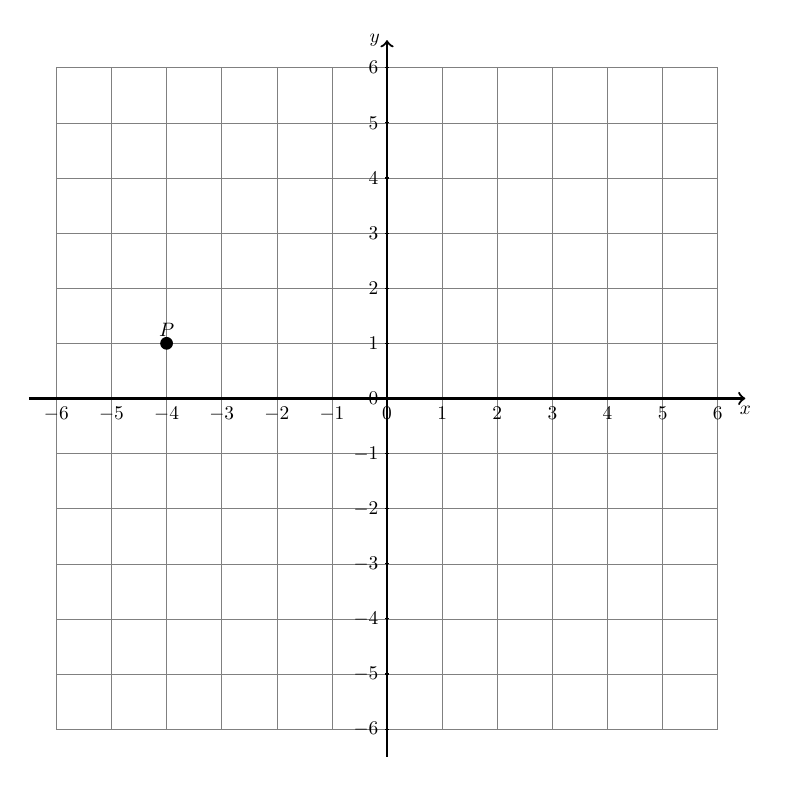
\begin{tikzpicture}[scale=0.7, transform shape]
    \def\axisLimit{6}

    \draw[step=1cm,gray,very thin] (-\axisLimit,-\axisLimit) grid (\axisLimit,\axisLimit);

    \draw[thick,->] (-\axisLimit-0.5,0) -- (\axisLimit+0.5,0) node[anchor=north] {$x$};
    \draw[thick,->] (0,-\axisLimit-0.5) -- (0,\axisLimit+0.5) node[anchor=east] {$y$};

    \foreach \x in {-\axisLimit,...,\axisLimit}
        \draw (\x cm,1pt) -- (\x cm,-1pt) node[anchor=north] {$\x$};
    \foreach \y in {-\axisLimit,...,\axisLimit}
        \draw (1pt,\y cm) -- (-1pt,\y cm) node[anchor=east] {$\y$};

    \filldraw[black] (-4,1) circle (3pt);
    \node[above] at (-4,1) {$P$};
\end{tikzpicture}
\end{center}

\noindent Between 06:00 and 06:10, the specimen moves according to the column vector
$\begin{pmatrix} 5 \\ -3 \end{pmatrix}$, taking it to point $Q$.\\
Between 06:10 and 06:20, the satellite's tracking system then reflects the recorded position in the line $x = 0$ (the $y$-axis), giving the final logged position $R$.

\begin{enumerate}
    \item[(a)] Find the coordinates of point $Q$, the specimen's position at 06:10.

    \vspace{3cm}
    \answercoord{2}

    \item[(b)] Find the coordinates of point $R$, the logged position.

    \vspace{3.5cm}
    \answercoord{2}
\end{enumerate}
\end{question}
